\section{Implementazione}
\titleslide{Implementazione}
\subsection{Basis1DAbstract}
\begin{frame}
 \frametitle{Basis1DAbstract}
 \framesubtitle{Una classe astratta per risolvere i sottoproblemi agli autovalori}
 \begin{columns}
  \begin{column}{0.5\textwidth}
  Il problema viene sempre rimappato nell'intervallo $(0,1)$
 \begin{itemize}
  \item Calcola gli autovalori\\$\rightarrow$ \texttt{Next()}
  \item Valuta le funzioni di base\\$\rightarrow$ \texttt{EvaluateBasis(...)}
 \end{itemize}
  \end{column}
\begin{column}{0.5\textwidth}
 \begin{figure}
  \centering
  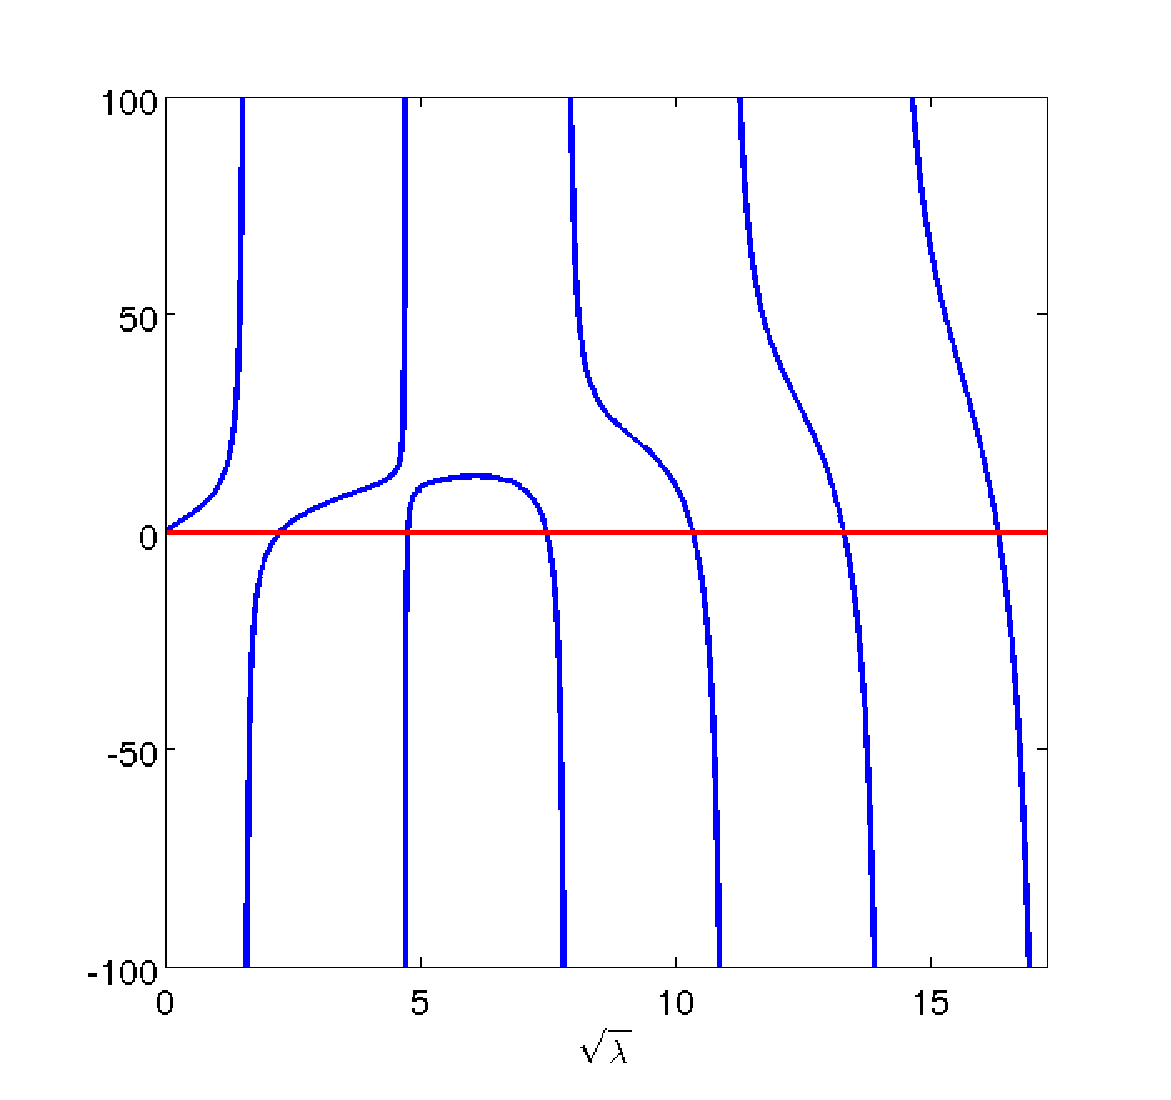
\includegraphics[scale=0.3,trim=1cm 1cm 1cm 1cm,clip=true]{Varie/ricercazeri}
 \end{figure}
\begin{center}Ricerca degli zeri con condizioni di Robin\end{center}
\end{column}
 \end{columns}
\end{frame}
\begin{frame}
 \frametitle{Polimorfismo su \texttt{Basis1DAbstract}...}
 \framesubtitle{... e su \texttt{EducatedBasisFunctorAbstract}}
 \begin{columns}
  \begin{column}{0.5\textwidth}
 \begin{figure}
  \centering
  {\linkimage{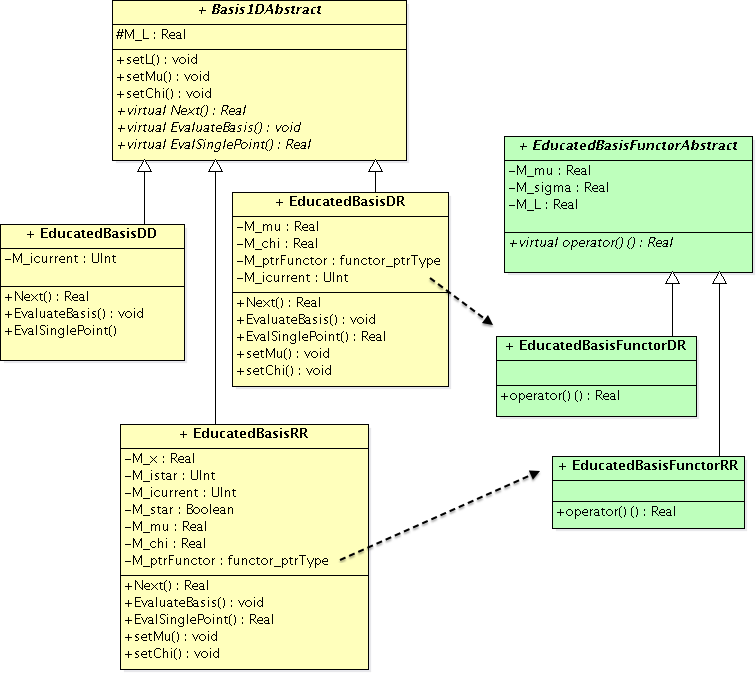
\includegraphics[scale=0.2]{UML/Basis1DAbstract}}{UML/Basis1DAbstract}}
 \end{figure}
  \end{column}
  \begin{column}{0.5\textwidth}
   Per gestire le diverse classi figlie di \texttt{Basis1DAbstract} abbiamo utilizzato una \textbf{factory}.
  \end{column}
 \end{columns}
\end{frame}
\subsection{ModalSpace}
\begin{frame}
 \frametitle{\texttt{ModalSpace}}
 \framesubtitle{Una classe che gestisce la costruzione dell'intera base modale}
 \begin{itemize}
  \item Gestisce le formule di quadratura sulla slice
  \item Istanzia i corretti generatori di base\\
  $\rightarrow$ \texttt{AddSliceBC(...)}
  \item Calcola gli autovalori del problema 2D\\
  $\rightarrow$ \texttt{EigensProvider(...)}
  \item Valuta le funzioni di base e le loro derivate nei nodi di quadratura\\
  $\rightarrow$ \texttt{??}
  \item Calcola i coefficient $r^{st}_{k,j}$\\
  $\rightarrow$ \texttt{Compute\_\*(...)}
 \end{itemize}
\end{frame}
\begin{frame}[fragile]
\frametitle{\texttt{AddSliceBC(...)}}
\framesubtitle{due metodi uno per ogni direzione}
\begin{lstlisting}[style = general]
void ModalSpace::
AddSliceBCY (const string& left, const string& right, const Real& mu, const Real& chi)
{
	// Creation of the correct basis generator
	M_genbasisY = Basis1DFactory::istance().createObject(left+right);
	// Setting of the parameters
	M_genbasisY->setL(M_Ly);
	M_genbasisY->setMu(mu);
	M_genbasisY->setChi(chi);
	return;
}
\end{lstlisting}
\end{frame}

\begin{frame}
 \frametitle{EigensProvider()}
 \framesubtitle{Ordinare correttamente gli autovalori non \`e facile}
 Una visualizzazione dell'algoritmo ad albero
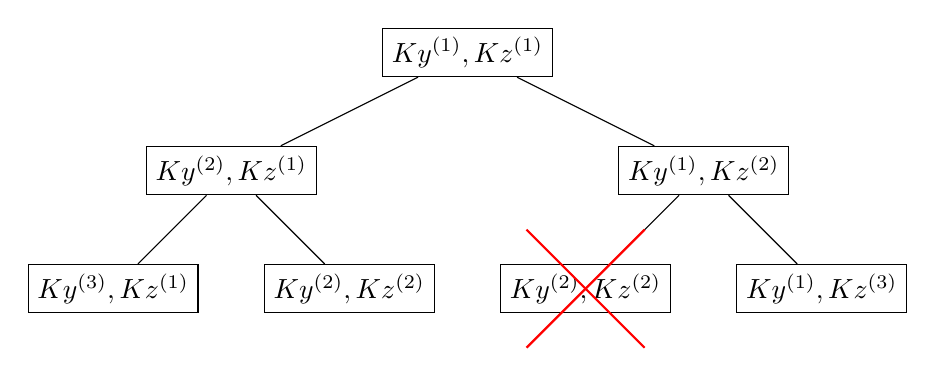
\begin{tikzpicture}
[scale=1.5]
\tikzstyle{every node}=[draw,shape=rectangle];
\path (5,0)  node (v1) {$Ky^{(1)},Kz^{(1)}$};
\path (3,-1) node (v2) {$Ky^{(2)},Kz^{(1)}$};
\path (7,-1) node (v3) {$Ky^{(1)},Kz^{(2)}$};
\path (2,-2) node (v4) {$Ky^{(3)},Kz^{(1)}$};
\path (4,-2) node (v5) {$Ky^{(2)},Kz^{(2)}$};
\path (6,-2) node (v6) {$Ky^{(2)},Kz^{(2)}$};
\path (8,-2) node (v7) {$Ky^{(1)},Kz^{(3)}$};
\draw (v1) -- (v2)
(v1) -- (v3)
(v2) -- (v4)
(v2) -- (v5)
(v3) -- (v6)
(v3) -- (v7);
\draw [thick,red, -] (5.5,-1.5)--(6.5,-2.5);
\draw [thick,red, -] (6.5,-1.5)--(5.5,-2.5);
\end{tikzpicture}
\end{frame}


\subsection{HiModAssembler}